\documentclass[12pt]{article}
\usepackage{newclude}
\usepackage[utf8]{inputenc}
\usepackage[acronym, toc]{glossaries}
\usepackage{amsmath,amsthm}
\usepackage{amssymb,amsfonts,latexsym,cancel}
\usepackage{graphicx}
\usepackage{float}
\usepackage{subfig}
\usepackage[normalem]{ulem}
\usepackage[lmargin=3cm,rmargin=3cm,top=2.5cm,bottom=2.5cm]{geometry}
\usepackage{longtable}
\usepackage{ragged2e}
\usepackage{datetime}
\usepackage{siunitx}
\usepackage{tikz}
\usetikzlibrary{shapes, positioning}
\usepackage{parskip}
\usepackage{fancyhdr}
\usepackage{titling}
\pagestyle{fancy}
\setlength{\headheight}{15.71667pt}
\usepackage{hyperref}
\hypersetup{
    colorlinks,
    citecolor=black,
    filecolor=black,
    linkcolor=black,
    urlcolor=black
}

\usepackage[
  backend=biber,
  style=ieee,
  url=false,
  doi=true,
  isbn=false
]{biblatex}
\addbibresource{bibliography.bib}

\includeonly{
    Introduction,
    Perspective,
    Homographies,
    Panoramic,
    Dental
}

\fancyfoot{}
\renewcommand{\footrulewidth}{0.5pt}
\fancyfoot[R]{\thepage}

\title{ Projective geometry and Panoramic image % Título de la práctica
}

\author{ Sergio Marín Sánchez % Nombre del autor
}
\newdate{date}{2}{4}{2024} % Fecha

\begin{document}
\begin{titlepage}
    \centering
    \phantom{a}
    \vspace{2cm}
    {
\includegraphics[scale=0.9]{ESCUDO_UPM.pdf}\par}
    \vspace{2cm}
    {\bfseries\LARGE Universidad Politécnica de Madrid \par}
    \vspace{0.75cm}
    {\scshape\Large Escuela Técnica Superior de Ingenieros Informáticos \par}
    \vfill
    {\scshape\Huge \thetitle \par}
    {\scshape\Large Image Processing, Analysis and Classification \par}
    \vfill
    {\large Author: \theauthor \par}
    \vspace{0.2cm}
    {\large Date: \displaydate{date} \par}
\end{titlepage}

\pagestyle{empty}
\tableofcontents
\clearpage

\setcounter{page}{1}

\pagestyle{fancy}

\section{Introduction}

\begin{frame}{\secname}{3D world $\rightarrow$ 2D content}
    An image is just a flat representation of the 3D world.
    \begin{figure}
        \centering
        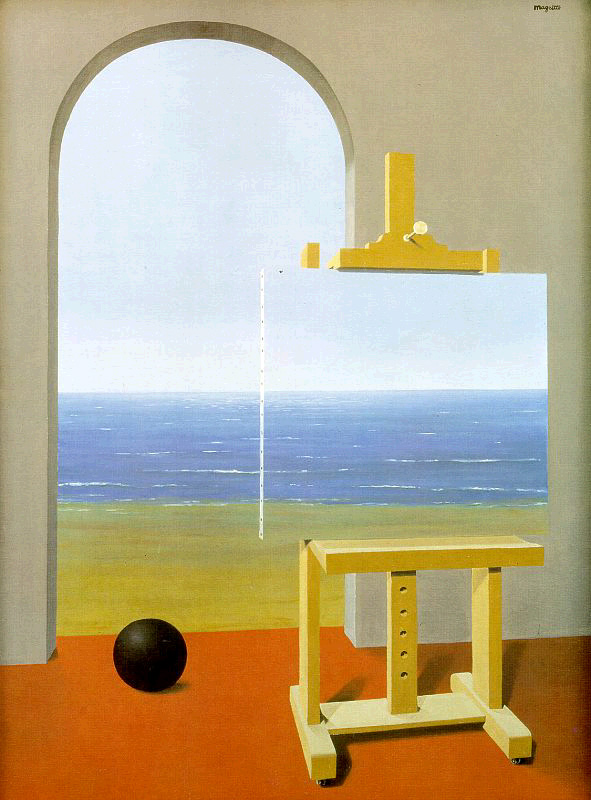
\includegraphics[height=0.5\textheight]{img/Magritte-human-condition.jpg}
    \end{figure}
    Even though we lose the depth component the image maintain the perspective.
\end{frame}

\begin{frame}{\secname}{3D world $\rightarrow$ 2D content}
    Image are useful to store memories, but also we can extract information from them. For instance, we may want to know how tall is this bottle.
    \begin{figure}
        \centering
        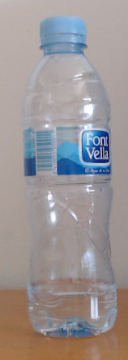
\includegraphics[height=0.5\textheight]{img/agua.png}
    \end{figure}
\end{frame}

\begin{frame}{\secname}{3D world $\rightarrow$ 2D content}
    We need to represent the images in such a way that both humans and computers are able to deal with them. Thus matrix representation of images is defined. We can define an image $I \in M_{h,w}\left(\mathbb{Z}^n\right)$ as:
    \begin{gather*}
        I = \begin{pmatrix}
            p_{1,1} & p_{1,2} & \dots & p_{1,w} \\
            p_{2,1} & p_{2,2} & \dots & p_{2,w} \\
            \vdots & \vdots & \ddots & \vdots \\
            p_{h,1} & p_{h,2} & \dots & p_{h,w} \\
        \end{pmatrix}_{h \times w}
    \end{gather*}
    
    Where each $p_{ij}$ is a vector in $\mathbb{Z}^n$, $n$ varies depending on the number of color channels.
\end{frame}

\begin{frame}{\secname}{3D world $\rightarrow$ 2D content}  
    Here we can see how the image is codified as we have defined before:
    \begin{figure}
        \centering
        \subfloat{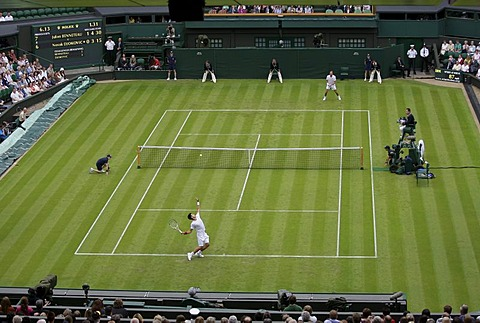
\includegraphics[width=0.4\textwidth]{img/tennis.jpg}}
        \qquad
        \subfloat{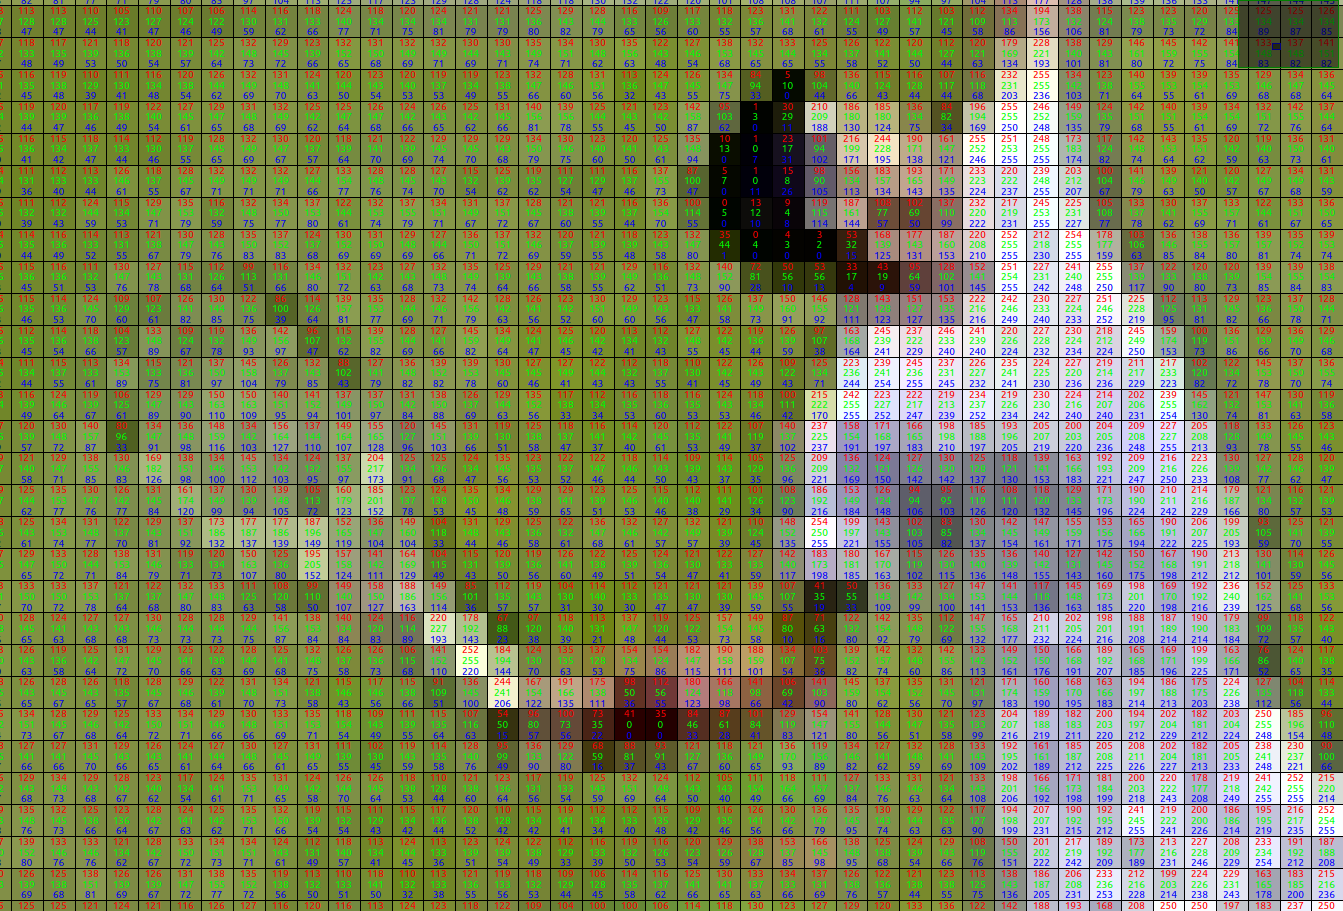
\includegraphics[width=0.4\textwidth]{img/pixels2.png}}
    \end{figure}
\end{frame}



\section{Perspective}

Perspective in digital images is a critical aspect that influences the perception of depth and spatial relationships within a scene. It is primarily manipulated through various parameters, with focal distance being one of the key elements.

The focal distance, often denoted as $f$, is a fundamental parameter in digital imaging that determines the magnification and perspective of the captured scene. It refers to the distance between the lens and the image sensor when the subject is in focus. A shorter focal distance results in a wider field of view, allowing more of the scene to be captured within the frame, while a longer focal distance narrows the field of view, resulting in magnification and compression of distant objects.

By using this focal distance, we can establish different measurements (angles) inside of the image. A potential use case for these measurements is triangulate locations. Firstly, some reference points are selected. Then, calculate the angle between them, two by two. Finally, these angles are placed over a map, and the intersection between them would indicate the actual position where the photo was taken. This method only requires some basic trigonometrics, as it can be seen in Fig. \ref{fig:triangulation}.

\begin{figure}[H]
    \centering
    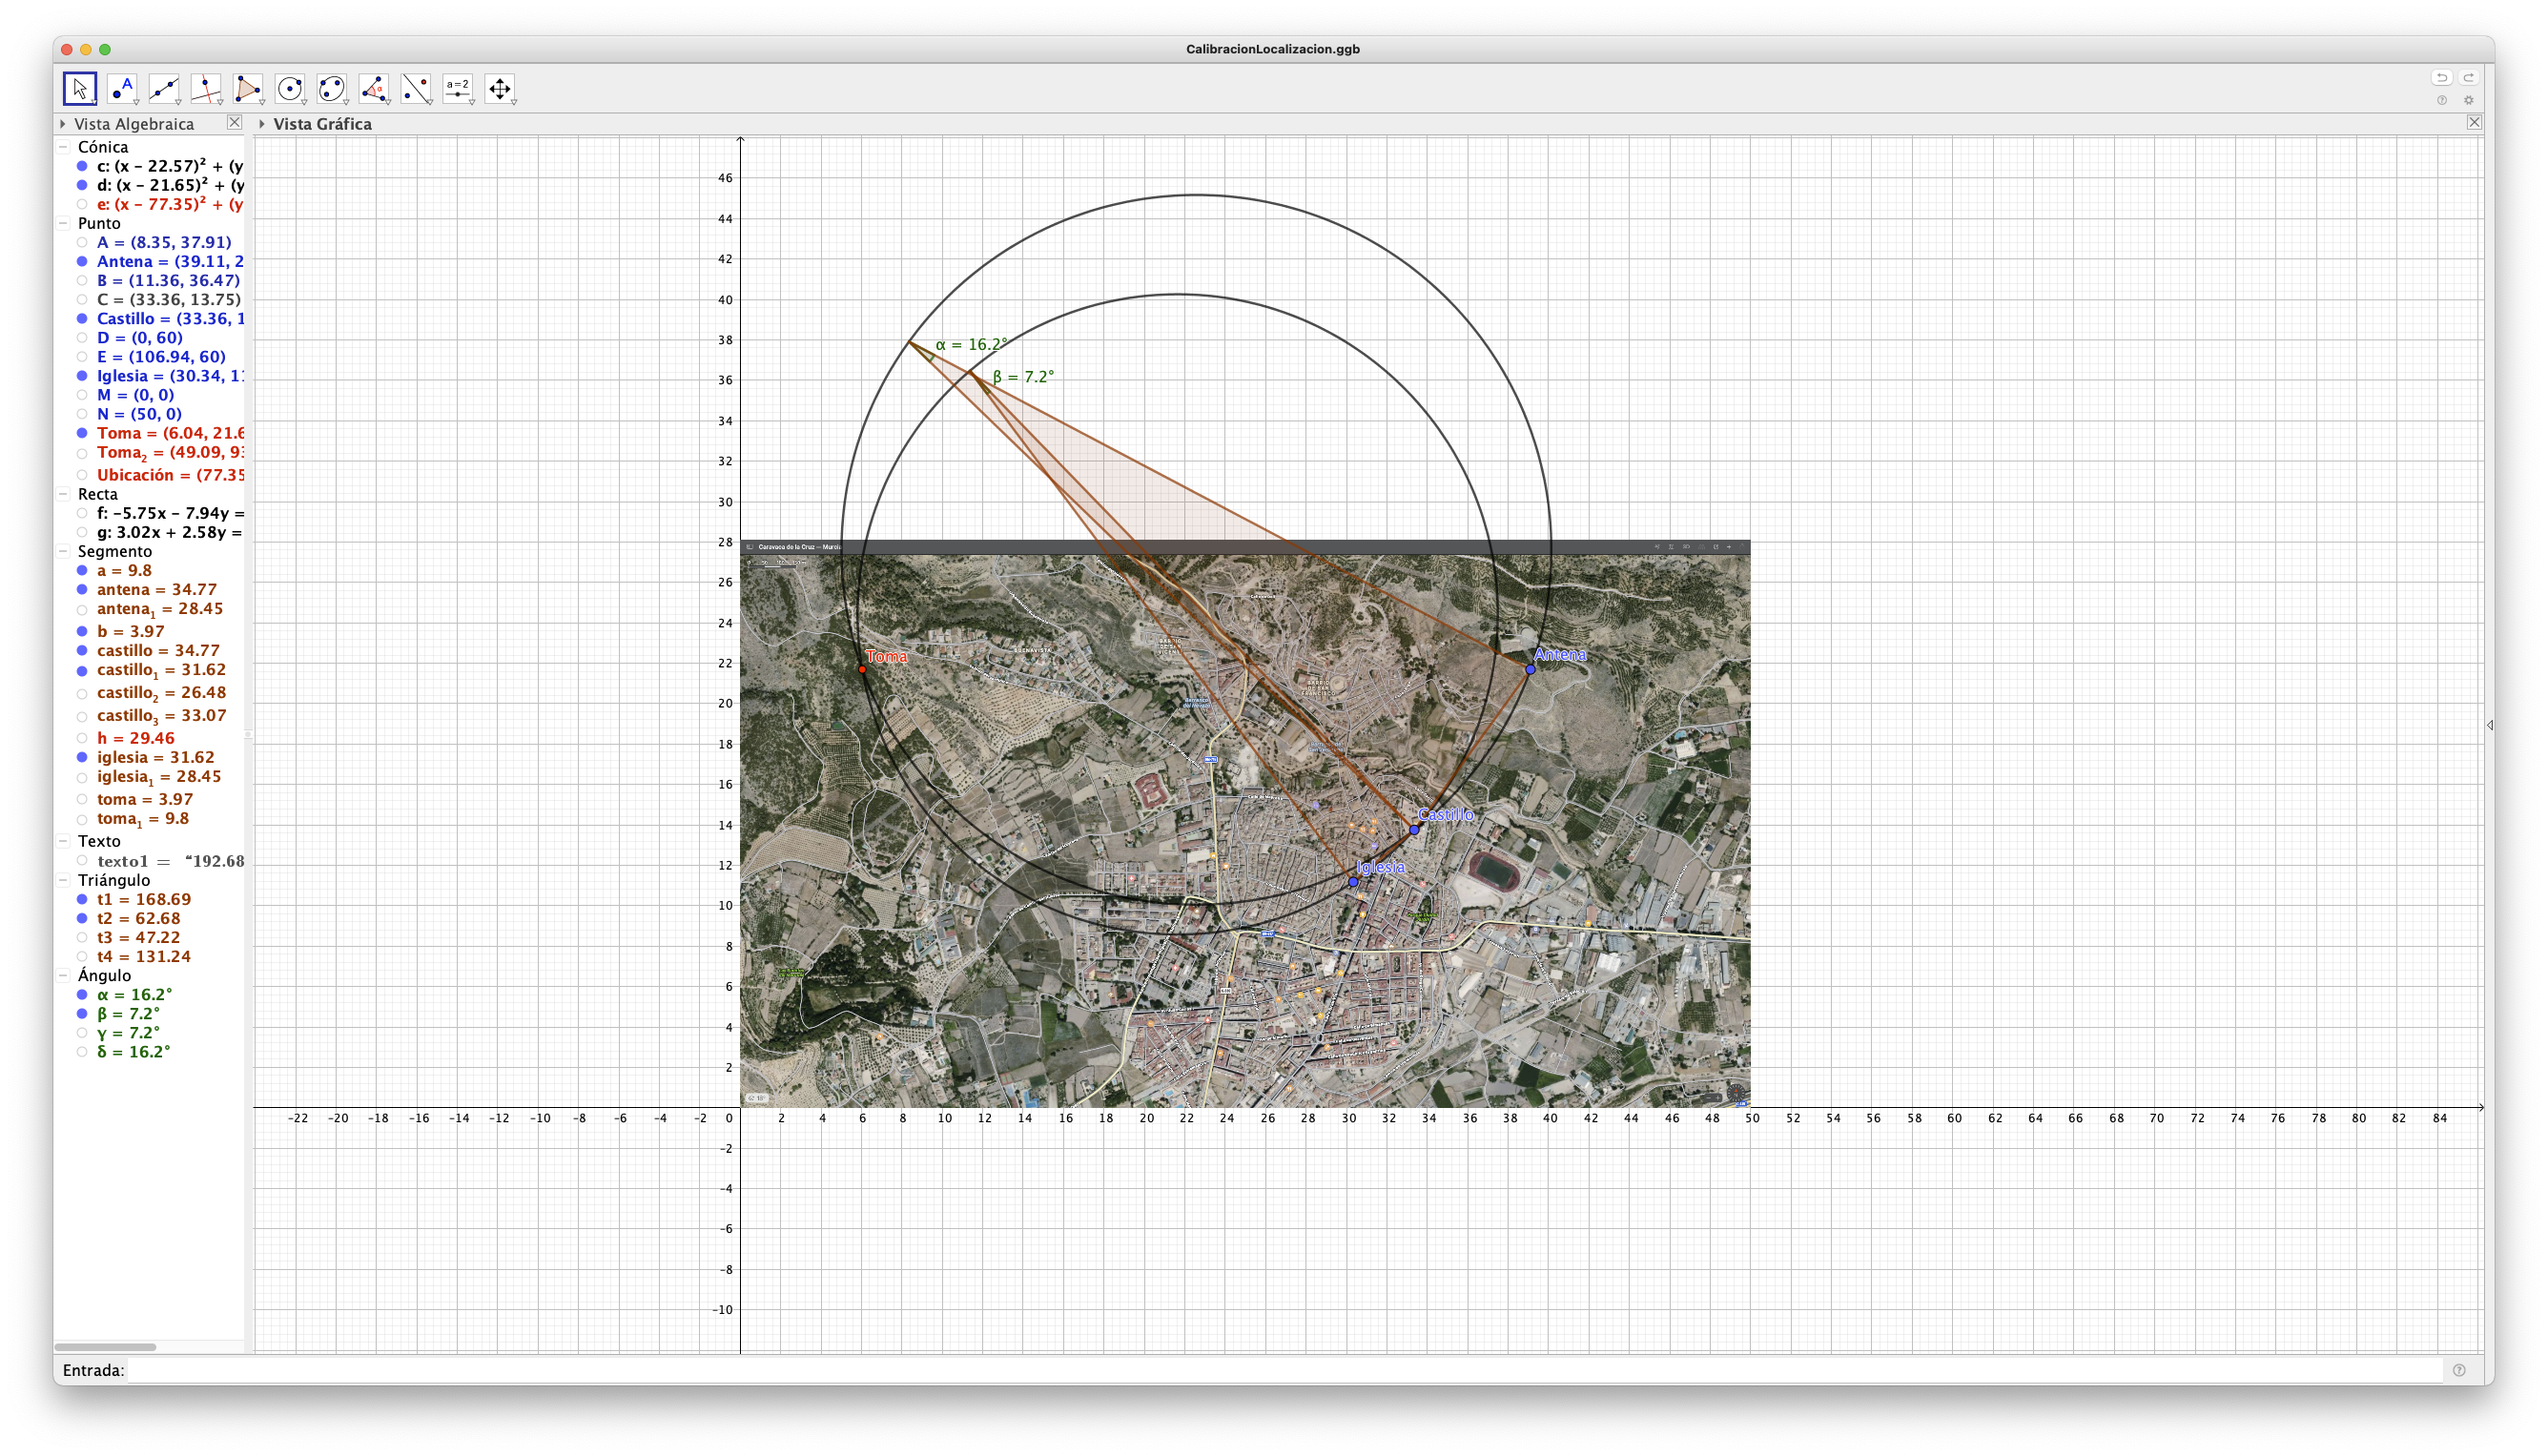
\includegraphics[width=0.9\textwidth]{img/Inter-Circs.png}
    \caption{Example of location triangulation}
    \label{fig:triangulation}
\end{figure}



\include*{Homographies}

\include*{Panoramic}

\include*{Dental}

\clearpage

\pagestyle{empty}
\renewcommand{\thepage}{}t

\nocite{*}

\printbibliography[heading=bibintoc]

\end{document}
